\newpage
\section{Resultados}

\subsection{Caso 1}

	Para o experimento 1, Vi foi mantida em 20V e Vo em 30V e a tabela \ref{t_rend1} sumariza os resultados obtidos.

	A razão cíclica utilizada foi de $D_1 = 37 \%$. Sendo a assim, o ganho teórico é de

	\[
		G_{teorico} = \frac{1}{1-D} = \frac{1}{1-0.37} = 1.5873 \cong 159 \%.
	\]

	O ganho médio, obtido a partir da tabela \ref{t_rend1}, é de
	
	\[
		G_{medio} = 153.29 \%.
	\]

	A diferença entre o ganho teórico ideal e o ganho médio medido se deve as perdas nos componentes e cabos do sistema. Como não ouve compensação da razão cíclica durante o experimento, essas perdas refletiram em quedas de tensão na entrada e saída do sistema.
	
	\begin{small}
		\begin{table}[H]
			\begin{center}
				\caption{Rendimento caso 1.}
				\begin{tabular}{l|l|l|l|l|l}
					\hline
					Tensão de   &  Corrente de 	& Tensão de & Corrente de	& Rendimento [\%] 	& Ganho    	\\
					entrada [V] &  entrada [A] 	& saída [V] & saída [A]  	&                 	& Estático 	\\
					\hline
					19.80 		& 1.04			& 30.3		& 0.60			& 88.2867			& 1.5303	\\
					\hline
					19.7		& 1.75			& 30.0		& 1.01			& 87.8898			& 1.5228	\\
					\hline
					19.6		& 2.65			& 29.8		& 1.52			& 87.2083			& 1.5204	\\
					\hline
					19.5		& 3.69			& 29.9		& 2.08			& 86.4318			& 1.5333	\\
					\hline
					19.4		& 4.58			& 29.9		& 2.54			& 85.4747			& 1.5412	\\
					\hline
					19.3		& 5.62			& 29.9		& 3.07			& 84.6284			& 1.5492	\\
				\end{tabular}
				\label{t_rend1}
			\end{center}
		\end{table}
	\end{small}

	A figura \ref{f_rend1} mostra o gráfico do rendimento para o caso 1, onde é possível observar que o rendimento diminui com o aumento da potência de saída.
	
	\begin{figure}[H]
		\centering
		\caption{Curva do rendimento para o caso 1.}
		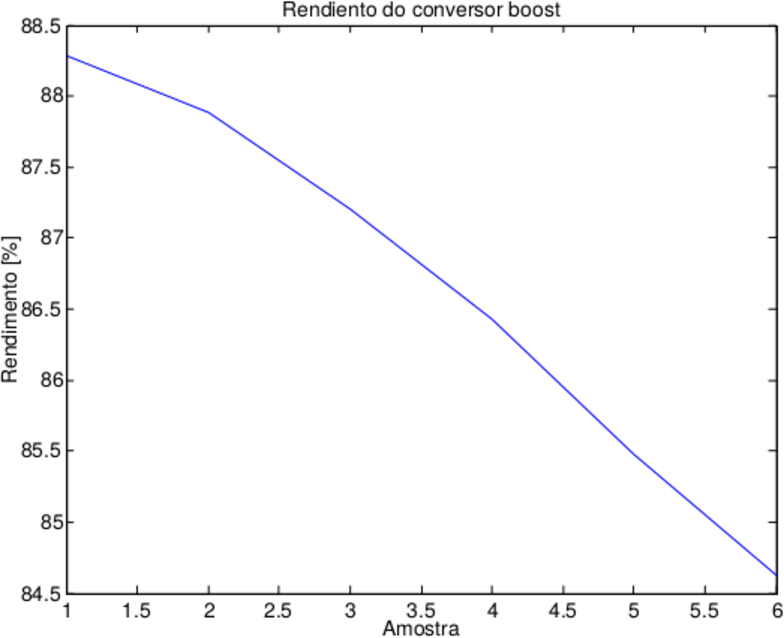
\includegraphics[scale=0.75]{rendimento1}
		\label{f_rend1}
	\end{figure}
	
\subsection{Caso 2}

	Para o experimento 2, Vi foi mantida em 20V e Vo em 40V e a tabela \ref{t_rend2} sumariza os resultados obtidos.
	
	A razão cíclica utilizada foi de $D_1 = 55 \%$. Sendo a assim, o ganho teórico é de
	
	\[
	G_{teorico} = \frac{1}{1-D} = \frac{1}{1-0.55} = 2.2222 \cong 222 \%.
	\]
	
	O ganho médio, obtido a partir da tabela \ref{t_rend2}, é de
	
	\[
	G_{medio} = 205.86 \%.
	\]
	
	A diferença entre o ganho teórico ideal e o ganho médio medido se deve as perdas nos componentes e cabos do sistema. Como não ouve compensação da razão cíclica durante o experimento, essas perdas refletiram em quedas de tensão na entrada e saída do sistema. Note que, como a potência de saída é maior que a do caso 1, as perdas no circuito também são maiores.
	
	\begin{small}
		\begin{table}[H]
			\begin{center}
				\caption{Rendimento caso 2.}
				\begin{tabular}{l|l|l|l|l|l}
					\hline
					Tensão de   &  Corrente de 	& Tensão de & Corrente de	& Rendimento [\%] 	& Ganho    	\\
					entrada [V] &  entrada [A] 	& saída [V] & saída [A]  	&                 	& Estático 	\\
					\hline
					19.6 		& 1.77			& 39.8		& 0.78			& 89.4846			& 2.0306	\\
					\hline
					19.5		& 2.30			& 39.9		& 1.01			& 89.8528			& 2.0462	\\
					\hline
					19.4		& 3.53			& 39.9		& 1.54			& 89.7258			& 2.0567	\\
					\hline
					19.3		& 4.79			& 39.9		& 2.05			& 88.4777			& 2.0674	\\
					\hline
					19.2		& 5.99			& 40.0		& 2.53			& 87.9939			& 2.0833	\\
					\hline
					19.2		& 6.38			& 39.7		& 2.57			& 83.2917			& 2.0677	\\
				\end{tabular}
				\label{t_rend2}
			\end{center}
		\end{table}
	\end{small}
	
	A figura \ref{f_rend2} mostra o gráfico do rendimento para o caso 2, onde é possível observar que, diferente do caso 1, o rendimento atinge um ponto máximo para corrente de saída de 1.01 A e, a partir daí, começa a diminuir.
	
	\begin{figure}[H]
		\centering
		\caption{Curva do rendimento para o caso 2.}
		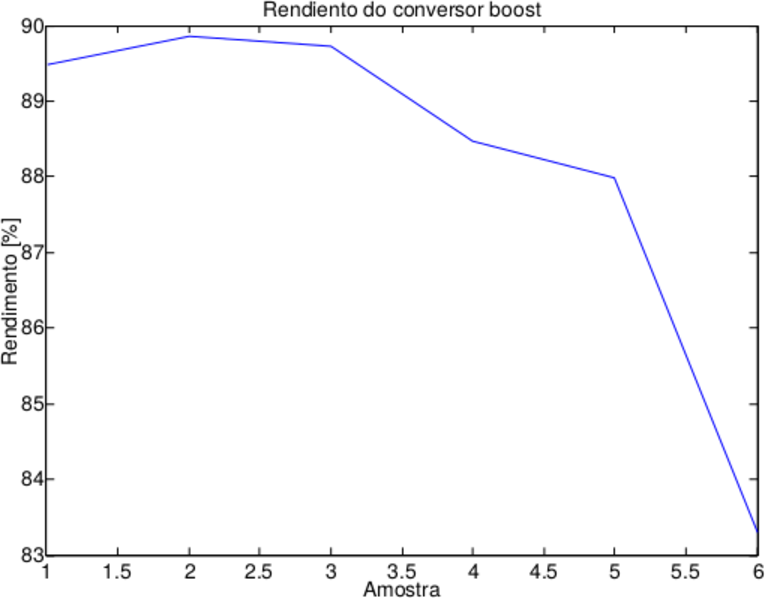
\includegraphics[scale=0.75]{rendimento2}
		\label{f_rend2}
	\end{figure}
	
\subsection{Perda}

	A figura \ref{f_perda} mostra a perda (em \textit{Watts}) em ambos os casos.

	\begin{figure}[H]
		\centering
		\caption{Perda em ambos os casos.}
		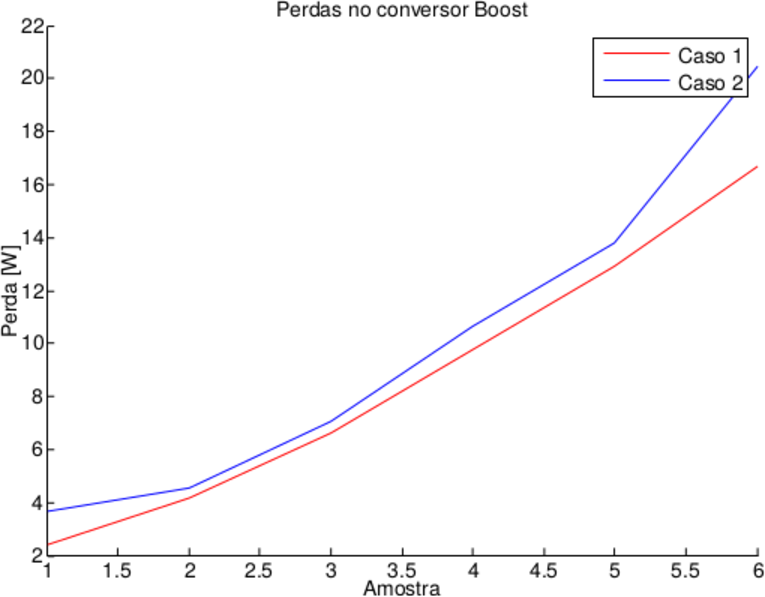
\includegraphics[scale=0.75]{perda}
		\label{f_perda}
	\end{figure}
	
	É notório que o conversor possui uma região de conversão onde a perda é minimizada.
	
\subsection{Forma de onda da tensão de saída}

	\begin{figure}[H]
		\centering
		\caption{Fora de onda na saída do caso 2.}
		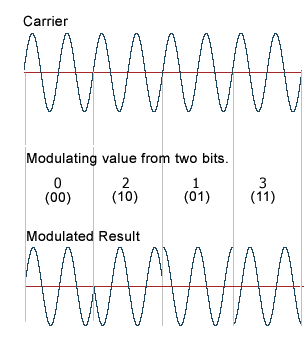
\includegraphics[scale=0.1]{onda}
		\label{f_onda}
	\end{figure}
	
	Como pode ser observado na figura \ref{f_onda}, a tensão de saída possui oscilações de alta frequência devido as componentes parasitas dos componentes. Estas oscilações aparecem amplificadas devido as características da ponteira do osciloscópio utilizado, sendo bem menores na carga. 